\documentclass[twoside]{book}

% Packages required by doxygen
\usepackage{fixltx2e}
\usepackage{calc}
\usepackage{doxygen}
\usepackage[export]{adjustbox} % also loads graphicx
\usepackage{graphicx}
\usepackage[utf8]{inputenc}
\usepackage{makeidx}
\usepackage{multicol}
\usepackage{multirow}
\PassOptionsToPackage{warn}{textcomp}
\usepackage{textcomp}
\usepackage[nointegrals]{wasysym}
\usepackage[table]{xcolor}

% Font selection
\usepackage[T1]{fontenc}
\usepackage[scaled=.90]{helvet}
\usepackage{courier}
\usepackage{amssymb}
\usepackage{sectsty}
\renewcommand{\familydefault}{\sfdefault}
\allsectionsfont{%
  \fontseries{bc}\selectfont%
  \color{darkgray}%
}
\renewcommand{\DoxyLabelFont}{%
  \fontseries{bc}\selectfont%
  \color{darkgray}%
}
\newcommand{\+}{\discretionary{\mbox{\scriptsize$\hookleftarrow$}}{}{}}

% Page & text layout
\usepackage{geometry}
\geometry{%
  a4paper,%
  top=2.5cm,%
  bottom=2.5cm,%
  left=2.5cm,%
  right=2.5cm%
}
\tolerance=750
\hfuzz=15pt
\hbadness=750
\setlength{\emergencystretch}{15pt}
\setlength{\parindent}{0cm}
\setlength{\parskip}{3ex plus 2ex minus 2ex}
\makeatletter
\renewcommand{\paragraph}{%
  \@startsection{paragraph}{4}{0ex}{-1.0ex}{1.0ex}{%
    \normalfont\normalsize\bfseries\SS@parafont%
  }%
}
\renewcommand{\subparagraph}{%
  \@startsection{subparagraph}{5}{0ex}{-1.0ex}{1.0ex}{%
    \normalfont\normalsize\bfseries\SS@subparafont%
  }%
}
\makeatother

% Headers & footers
\usepackage{fancyhdr}
\pagestyle{fancyplain}
\fancyhead[LE]{\fancyplain{}{\bfseries\thepage}}
\fancyhead[CE]{\fancyplain{}{}}
\fancyhead[RE]{\fancyplain{}{\bfseries\leftmark}}
\fancyhead[LO]{\fancyplain{}{\bfseries\rightmark}}
\fancyhead[CO]{\fancyplain{}{}}
\fancyhead[RO]{\fancyplain{}{\bfseries\thepage}}
\fancyfoot[LE]{\fancyplain{}{}}
\fancyfoot[CE]{\fancyplain{}{}}
\fancyfoot[RE]{\fancyplain{}{\bfseries\scriptsize Generated by Doxygen }}
\fancyfoot[LO]{\fancyplain{}{\bfseries\scriptsize Generated by Doxygen }}
\fancyfoot[CO]{\fancyplain{}{}}
\fancyfoot[RO]{\fancyplain{}{}}
\renewcommand{\footrulewidth}{0.4pt}
\renewcommand{\chaptermark}[1]{%
  \markboth{#1}{}%
}
\renewcommand{\sectionmark}[1]{%
  \markright{\thesection\ #1}%
}

% Indices & bibliography
\usepackage{natbib}
\usepackage[titles]{tocloft}
\setcounter{tocdepth}{3}
\setcounter{secnumdepth}{5}
\makeindex

% Hyperlinks (required, but should be loaded last)
\usepackage{ifpdf}
\ifpdf
  \usepackage[pdftex,pagebackref=true]{hyperref}
\else
  \usepackage[ps2pdf,pagebackref=true]{hyperref}
\fi
\hypersetup{%
  colorlinks=true,%
  linkcolor=blue,%
  citecolor=blue,%
  unicode%
}

% Custom commands
\newcommand{\clearemptydoublepage}{%
  \newpage{\pagestyle{empty}\cleardoublepage}%
}

\usepackage{caption}
\captionsetup{labelsep=space,justification=centering,font={bf},singlelinecheck=off,skip=4pt,position=top}

%===== C O N T E N T S =====

\begin{document}

% Titlepage & ToC
\hypersetup{pageanchor=false,
             bookmarksnumbered=true,
             pdfencoding=unicode
            }
\pagenumbering{roman}
\begin{titlepage}
\vspace*{7cm}
\begin{center}%
{\Large terrapinavigator \\[1ex]\large 1.\+0 }\\
\vspace*{1cm}
{\large Generated by Doxygen 1.8.11}\\
\end{center}
\end{titlepage}
\clearemptydoublepage
\tableofcontents
\clearemptydoublepage
\pagenumbering{arabic}
\hypersetup{pageanchor=true}

%--- Begin generated contents ---
\chapter{Class Index}
\section{Class List}
Here are the classes, structs, unions and interfaces with brief descriptions\+:\begin{DoxyCompactList}
\item\contentsline{section}{\hyperlink{classNavigator}{Navigator} \\*\hyperlink{classNavigator}{Navigator} class }{\pageref{classNavigator}}{}
\item\contentsline{section}{\hyperlink{classTerpCam}{Terp\+Cam} \\*\hyperlink{classTerpCam}{Terp\+Cam} class }{\pageref{classTerpCam}}{}
\item\contentsline{section}{\hyperlink{classTurtle}{Turtle} \\*\hyperlink{classTurtle}{Turtle} class }{\pageref{classTurtle}}{}
\end{DoxyCompactList}

\chapter{File Index}
\section{File List}
Here is a list of all documented files with brief descriptions\+:\begin{DoxyCompactList}
\item\contentsline{section}{include/terrapinavigator/\hyperlink{Navigator_8h}{Navigator.\+h} \\*Header file of \hyperlink{classNavigator}{Navigator} class }{\pageref{Navigator_8h}}{}
\item\contentsline{section}{include/terrapinavigator/\hyperlink{TerpCam_8h}{Terp\+Cam.\+h} \\*Header file for \hyperlink{classTerpCam}{Terp\+Cam} class }{\pageref{TerpCam_8h}}{}
\item\contentsline{section}{include/terrapinavigator/\hyperlink{Turtle_8h}{Turtle.\+h} \\*Header File for turtle Class }{\pageref{Turtle_8h}}{}
\item\contentsline{section}{src/\hyperlink{main_8cpp}{main.\+cpp} \\*Demo for the project }{\pageref{main_8cpp}}{}
\item\contentsline{section}{src/\hyperlink{Navigator_8cpp}{Navigator.\+cpp} \\*Implementation of \hyperlink{classNavigator}{Navigator} class }{\pageref{Navigator_8cpp}}{}
\item\contentsline{section}{src/\hyperlink{TerpCam_8cpp}{Terp\+Cam.\+cpp} \\*Implementation of \hyperlink{classTerpCam}{Terp\+Cam} class }{\pageref{TerpCam_8cpp}}{}
\item\contentsline{section}{src/\hyperlink{Turtle_8cpp}{Turtle.\+cpp} \\*Implementation of \hyperlink{classTurtle}{Turtle} class }{\pageref{Turtle_8cpp}}{}
\item\contentsline{section}{test/\hyperlink{NavigatorTest_8cpp}{Navigator\+Test.\+cpp} \\*Contains tests for navigator class }{\pageref{NavigatorTest_8cpp}}{}
\item\contentsline{section}{test/\hyperlink{TerpCamTest_8cpp}{Terp\+Cam\+Test.\+cpp} \\*Contains tests for \hyperlink{classTerpCam}{Terp\+Cam} class }{\pageref{TerpCamTest_8cpp}}{}
\item\contentsline{section}{test/\hyperlink{terpTest_8cpp}{terp\+Test.\+cpp} \\*Contains the main function to run all tests }{\pageref{terpTest_8cpp}}{}
\item\contentsline{section}{test/\hyperlink{TurtleTest_8cpp}{Turtle\+Test.\+cpp} \\*Contains tests for \hyperlink{classTurtle}{Turtle} class }{\pageref{TurtleTest_8cpp}}{}
\end{DoxyCompactList}

\chapter{Class Documentation}
\hypertarget{classNavigator}{}\section{Navigator Class Reference}
\label{classNavigator}\index{Navigator@{Navigator}}


\hyperlink{classNavigator}{Navigator} class.  




{\ttfamily \#include $<$Navigator.\+h$>$}

\subsection*{Public Member Functions}
\begin{DoxyCompactItemize}
\item 
\hyperlink{classNavigator_a59230ab4698882f754d5ce275a1a4030}{Navigator} ()\hypertarget{classNavigator_a59230ab4698882f754d5ce275a1a4030}{}\label{classNavigator_a59230ab4698882f754d5ce275a1a4030}

\begin{DoxyCompactList}\small\item\em constuctor for \hyperlink{classNavigator}{Navigator} Class \end{DoxyCompactList}\item 
float \hyperlink{classNavigator_aecf7698fab9b42b91ee387524a0d9284}{get\+Obst\+Dist} ()
\begin{DoxyCompactList}\small\item\em getter for obst\+Dist \end{DoxyCompactList}\item 
bool \hyperlink{classNavigator_a4d838ef75089c6dc9e2530e5f39a389e}{get\+Rotate\+Flag} ()
\begin{DoxyCompactList}\small\item\em getter for rotate\+Flag \end{DoxyCompactList}\item 
void \hyperlink{classNavigator_afe356293bdf38da88a426f161d969ad8}{set\+Rotate\+Flag} ()
\begin{DoxyCompactList}\small\item\em setter for rotate\+Flag \end{DoxyCompactList}\item 
void \hyperlink{classNavigator_afd068836c4f8c13a2d072f0bf249dc88}{Scan\+Callback} (const sensor\+\_\+msgs\+::\+Laser\+Scan\+::\+Const\+Ptr \&input)
\begin{DoxyCompactList}\small\item\em callback function for the camera subscriber \end{DoxyCompactList}\item 
void \hyperlink{classNavigator_a16dbd75e0fcc830c871b424af0a72938}{Rotatetimer\+Callback} (const ros\+::\+Timer\+Event \&event)
\begin{DoxyCompactList}\small\item\em callback function for the rotate timer \end{DoxyCompactList}\item 
geometry\+\_\+msgs\+::\+Twist \hyperlink{classNavigator_ad3924883d7b8edd7728510b2d466baa3}{dir} ()
\begin{DoxyCompactList}\small\item\em callback function for the cam timer \end{DoxyCompactList}\item 
\hyperlink{classNavigator_a81bb9c10588736497700032d8b61e9d1}{$\sim$\+Navigator} ()\hypertarget{classNavigator_a81bb9c10588736497700032d8b61e9d1}{}\label{classNavigator_a81bb9c10588736497700032d8b61e9d1}

\begin{DoxyCompactList}\small\item\em Destructor for \hyperlink{classNavigator}{Navigator} Class. \end{DoxyCompactList}\end{DoxyCompactItemize}


\subsection{Detailed Description}
\hyperlink{classNavigator}{Navigator} class. 

Generates twist messages for turtlebot to explore Starts by rotating in place then moving ahead Rotates in place every 45 seconds to aid mapping Avoids obstacles by rotating with random angles till clear 

\subsection{Member Function Documentation}
\index{Navigator@{Navigator}!dir@{dir}}
\index{dir@{dir}!Navigator@{Navigator}}
\subsubsection[{\texorpdfstring{dir()}{dir()}}]{\setlength{\rightskip}{0pt plus 5cm}geometry\+\_\+msgs\+::\+Twist Navigator\+::dir (
\begin{DoxyParamCaption}
{}
\end{DoxyParamCaption}
)}\hypertarget{classNavigator_ad3924883d7b8edd7728510b2d466baa3}{}\label{classNavigator_ad3924883d7b8edd7728510b2d466baa3}


callback function for the cam timer 

Generates twist messages for turtle\+Bot to moce

\begin{DoxyReturn}{Returns}
action (the twist messages) 
\end{DoxyReturn}
\index{Navigator@{Navigator}!get\+Obst\+Dist@{get\+Obst\+Dist}}
\index{get\+Obst\+Dist@{get\+Obst\+Dist}!Navigator@{Navigator}}
\subsubsection[{\texorpdfstring{get\+Obst\+Dist()}{getObstDist()}}]{\setlength{\rightskip}{0pt plus 5cm}float Navigator\+::get\+Obst\+Dist (
\begin{DoxyParamCaption}
{}
\end{DoxyParamCaption}
)}\hypertarget{classNavigator_aecf7698fab9b42b91ee387524a0d9284}{}\label{classNavigator_aecf7698fab9b42b91ee387524a0d9284}


getter for obst\+Dist 

\begin{DoxyReturn}{Returns}
obst\+Dist 
\end{DoxyReturn}
\index{Navigator@{Navigator}!get\+Rotate\+Flag@{get\+Rotate\+Flag}}
\index{get\+Rotate\+Flag@{get\+Rotate\+Flag}!Navigator@{Navigator}}
\subsubsection[{\texorpdfstring{get\+Rotate\+Flag()}{getRotateFlag()}}]{\setlength{\rightskip}{0pt plus 5cm}bool Navigator\+::get\+Rotate\+Flag (
\begin{DoxyParamCaption}
{}
\end{DoxyParamCaption}
)}\hypertarget{classNavigator_a4d838ef75089c6dc9e2530e5f39a389e}{}\label{classNavigator_a4d838ef75089c6dc9e2530e5f39a389e}


getter for rotate\+Flag 

\begin{DoxyReturn}{Returns}
rotate\+Flag 
\end{DoxyReturn}
\index{Navigator@{Navigator}!Rotatetimer\+Callback@{Rotatetimer\+Callback}}
\index{Rotatetimer\+Callback@{Rotatetimer\+Callback}!Navigator@{Navigator}}
\subsubsection[{\texorpdfstring{Rotatetimer\+Callback(const ros\+::\+Timer\+Event \&event)}{RotatetimerCallback(const ros::TimerEvent &event)}}]{\setlength{\rightskip}{0pt plus 5cm}void Navigator\+::\+Rotatetimer\+Callback (
\begin{DoxyParamCaption}
\item[{const ros\+::\+Timer\+Event \&}]{event}
\end{DoxyParamCaption}
)}\hypertarget{classNavigator_a16dbd75e0fcc830c871b424af0a72938}{}\label{classNavigator_a16dbd75e0fcc830c871b424af0a72938}


callback function for the rotate timer 

sets the take rotate flag to true every 45 seconds


\begin{DoxyParams}{Parameters}
{\em event} & is the ros\+::\+Timer\+Event structure it provides timing information useful when debugging.\\
\hline
\end{DoxyParams}
\begin{DoxyReturn}{Returns}
none 
\end{DoxyReturn}
\index{Navigator@{Navigator}!Scan\+Callback@{Scan\+Callback}}
\index{Scan\+Callback@{Scan\+Callback}!Navigator@{Navigator}}
\subsubsection[{\texorpdfstring{Scan\+Callback(const sensor\+\_\+msgs\+::\+Laser\+Scan\+::\+Const\+Ptr \&input)}{ScanCallback(const sensor_msgs::LaserScan::ConstPtr &input)}}]{\setlength{\rightskip}{0pt plus 5cm}void Navigator\+::\+Scan\+Callback (
\begin{DoxyParamCaption}
\item[{const sensor\+\_\+msgs\+::\+Laser\+Scan\+::\+Const\+Ptr \&}]{input}
\end{DoxyParamCaption}
)}\hypertarget{classNavigator_afd068836c4f8c13a2d072f0bf249dc88}{}\label{classNavigator_afd068836c4f8c13a2d072f0bf249dc88}


callback function for the camera subscriber 

finds the closest obstacle


\begin{DoxyParams}{Parameters}
{\em input} & is the pointer to array containing obstacle distances\\
\hline
\end{DoxyParams}
\begin{DoxyReturn}{Returns}
none 
\end{DoxyReturn}
\index{Navigator@{Navigator}!set\+Rotate\+Flag@{set\+Rotate\+Flag}}
\index{set\+Rotate\+Flag@{set\+Rotate\+Flag}!Navigator@{Navigator}}
\subsubsection[{\texorpdfstring{set\+Rotate\+Flag()}{setRotateFlag()}}]{\setlength{\rightskip}{0pt plus 5cm}void Navigator\+::set\+Rotate\+Flag (
\begin{DoxyParamCaption}
{}
\end{DoxyParamCaption}
)}\hypertarget{classNavigator_afe356293bdf38da88a426f161d969ad8}{}\label{classNavigator_afe356293bdf38da88a426f161d969ad8}


setter for rotate\+Flag 

sets the rotate\+Flag to false

\begin{DoxyReturn}{Returns}
none 
\end{DoxyReturn}


The documentation for this class was generated from the following files\+:\begin{DoxyCompactItemize}
\item 
include/terrapinavigator/\hyperlink{Navigator_8h}{Navigator.\+h}\item 
src/\hyperlink{Navigator_8cpp}{Navigator.\+cpp}\end{DoxyCompactItemize}

\hypertarget{classTerpCam}{}\section{Terp\+Cam Class Reference}
\label{classTerpCam}\index{Terp\+Cam@{Terp\+Cam}}


\hyperlink{classTerpCam}{Terp\+Cam} class.  




{\ttfamily \#include $<$Terp\+Cam.\+h$>$}

\subsection*{Public Member Functions}
\begin{DoxyCompactItemize}
\item 
\hyperlink{classTerpCam_a447cd41ae2673fcb318f823c3624cf85}{Terp\+Cam} ()\hypertarget{classTerpCam_a447cd41ae2673fcb318f823c3624cf85}{}\label{classTerpCam_a447cd41ae2673fcb318f823c3624cf85}

\begin{DoxyCompactList}\small\item\em Destructor for \hyperlink{classTerpCam}{Terp\+Cam} Class. \end{DoxyCompactList}\item 
bool \hyperlink{classTerpCam_acfc8df6c8c13209279afe270cd55021d}{get\+Take\+Image\+Flag} ()
\begin{DoxyCompactList}\small\item\em getter for take\+Image\+Flag \end{DoxyCompactList}\item 
void \hyperlink{classTerpCam_ae61767e8357dfe8ceccdd04734e3e94d}{set\+Take\+Image\+Flag} ()
\begin{DoxyCompactList}\small\item\em setter for take\+Image\+Flag \end{DoxyCompactList}\item 
bool \hyperlink{classTerpCam_a17bb8fc53fd73ab9c4138b02eed3b62b}{take\+Image} (terrapinavigator\+::picture\+Service\+::\+Request \&req, terrapinavigator\+::picture\+Service\+::\+Response \&resp)
\begin{DoxyCompactList}\small\item\em callback function for the take image server \end{DoxyCompactList}\item 
void \hyperlink{classTerpCam_a7315af3e74448baf8ffa3d5d81020530}{cam\+Timer\+Callback} (const ros\+::\+Timer\+Event \&event)
\begin{DoxyCompactList}\small\item\em callback function for the cam timer \end{DoxyCompactList}\item 
void \hyperlink{classTerpCam_aa847acf259a1108ad7c15a92e0be291b}{camera\+Callback} (const sensor\+\_\+msgs\+::\+Image\+Const\+Ptr \&img)
\begin{DoxyCompactList}\small\item\em callback function for the camera subscriber \end{DoxyCompactList}\item 
\hyperlink{classTerpCam_abf1740200fd7d293b92d37ddcd8d4c43}{$\sim$\+Terp\+Cam} ()\hypertarget{classTerpCam_abf1740200fd7d293b92d37ddcd8d4c43}{}\label{classTerpCam_abf1740200fd7d293b92d37ddcd8d4c43}

\begin{DoxyCompactList}\small\item\em Destructor for \hyperlink{classTerpCam}{Terp\+Cam} Class. \end{DoxyCompactList}\end{DoxyCompactItemize}


\subsection{Detailed Description}
\hyperlink{classTerpCam}{Terp\+Cam} class. 

Implements picture service Takes a picture every 40 seconds Also can take pictures when desired by the user 

\subsection{Member Function Documentation}
\index{Terp\+Cam@{Terp\+Cam}!camera\+Callback@{camera\+Callback}}
\index{camera\+Callback@{camera\+Callback}!Terp\+Cam@{Terp\+Cam}}
\subsubsection[{\texorpdfstring{camera\+Callback(const sensor\+\_\+msgs\+::\+Image\+Const\+Ptr \&img)}{cameraCallback(const sensor_msgs::ImageConstPtr &img)}}]{\setlength{\rightskip}{0pt plus 5cm}void Terp\+Cam\+::camera\+Callback (
\begin{DoxyParamCaption}
\item[{const sensor\+\_\+msgs\+::\+Image\+Const\+Ptr \&}]{img}
\end{DoxyParamCaption}
)}\hypertarget{classTerpCam_aa847acf259a1108ad7c15a92e0be291b}{}\label{classTerpCam_aa847acf259a1108ad7c15a92e0be291b}


callback function for the camera subscriber 

saves an image locally if take image flag is true


\begin{DoxyParams}{Parameters}
{\em img} & is a constant image pointer of what the turtlebot is seeing\\
\hline
\end{DoxyParams}
\begin{DoxyReturn}{Returns}
none 
\end{DoxyReturn}
\index{Terp\+Cam@{Terp\+Cam}!cam\+Timer\+Callback@{cam\+Timer\+Callback}}
\index{cam\+Timer\+Callback@{cam\+Timer\+Callback}!Terp\+Cam@{Terp\+Cam}}
\subsubsection[{\texorpdfstring{cam\+Timer\+Callback(const ros\+::\+Timer\+Event \&event)}{camTimerCallback(const ros::TimerEvent &event)}}]{\setlength{\rightskip}{0pt plus 5cm}void Terp\+Cam\+::cam\+Timer\+Callback (
\begin{DoxyParamCaption}
\item[{const ros\+::\+Timer\+Event \&}]{event}
\end{DoxyParamCaption}
)}\hypertarget{classTerpCam_a7315af3e74448baf8ffa3d5d81020530}{}\label{classTerpCam_a7315af3e74448baf8ffa3d5d81020530}


callback function for the cam timer 

sets the take image flag to true every 40 seconds


\begin{DoxyParams}{Parameters}
{\em event} & is the ros\+::\+Timer\+Event structure it provides timing information useful when debugging.\\
\hline
\end{DoxyParams}
\begin{DoxyReturn}{Returns}
none 
\end{DoxyReturn}
\index{Terp\+Cam@{Terp\+Cam}!get\+Take\+Image\+Flag@{get\+Take\+Image\+Flag}}
\index{get\+Take\+Image\+Flag@{get\+Take\+Image\+Flag}!Terp\+Cam@{Terp\+Cam}}
\subsubsection[{\texorpdfstring{get\+Take\+Image\+Flag()}{getTakeImageFlag()}}]{\setlength{\rightskip}{0pt plus 5cm}bool Terp\+Cam\+::get\+Take\+Image\+Flag (
\begin{DoxyParamCaption}
{}
\end{DoxyParamCaption}
)}\hypertarget{classTerpCam_acfc8df6c8c13209279afe270cd55021d}{}\label{classTerpCam_acfc8df6c8c13209279afe270cd55021d}


getter for take\+Image\+Flag 

\begin{DoxyReturn}{Returns}
take\+Image\+Flag 
\end{DoxyReturn}
\index{Terp\+Cam@{Terp\+Cam}!set\+Take\+Image\+Flag@{set\+Take\+Image\+Flag}}
\index{set\+Take\+Image\+Flag@{set\+Take\+Image\+Flag}!Terp\+Cam@{Terp\+Cam}}
\subsubsection[{\texorpdfstring{set\+Take\+Image\+Flag()}{setTakeImageFlag()}}]{\setlength{\rightskip}{0pt plus 5cm}void Terp\+Cam\+::set\+Take\+Image\+Flag (
\begin{DoxyParamCaption}
{}
\end{DoxyParamCaption}
)}\hypertarget{classTerpCam_ae61767e8357dfe8ceccdd04734e3e94d}{}\label{classTerpCam_ae61767e8357dfe8ceccdd04734e3e94d}


setter for take\+Image\+Flag 

sets the take\+Image\+Flag to true

\begin{DoxyReturn}{Returns}
none 
\end{DoxyReturn}
\index{Terp\+Cam@{Terp\+Cam}!take\+Image@{take\+Image}}
\index{take\+Image@{take\+Image}!Terp\+Cam@{Terp\+Cam}}
\subsubsection[{\texorpdfstring{take\+Image(terrapinavigator\+::picture\+Service\+::\+Request \&req, terrapinavigator\+::picture\+Service\+::\+Response \&resp)}{takeImage(terrapinavigator::pictureService::Request &req, terrapinavigator::pictureService::Response &resp)}}]{\setlength{\rightskip}{0pt plus 5cm}bool Terp\+Cam\+::take\+Image (
\begin{DoxyParamCaption}
\item[{terrapinavigator\+::picture\+Service\+::\+Request \&}]{req, }
\item[{terrapinavigator\+::picture\+Service\+::\+Response \&}]{resp}
\end{DoxyParamCaption}
)}\hypertarget{classTerpCam_a17bb8fc53fd73ab9c4138b02eed3b62b}{}\label{classTerpCam_a17bb8fc53fd73ab9c4138b02eed3b62b}


callback function for the take image server 


\begin{DoxyParams}{Parameters}
{\em \&req} & is the request sent by the client \\
\hline
{\em \&resp} & is the response sent by the server\\
\hline
\end{DoxyParams}
\begin{DoxyReturn}{Returns}
true if the response is successful 
\end{DoxyReturn}


The documentation for this class was generated from the following files\+:\begin{DoxyCompactItemize}
\item 
include/terrapinavigator/\hyperlink{TerpCam_8h}{Terp\+Cam.\+h}\item 
src/\hyperlink{TerpCam_8cpp}{Terp\+Cam.\+cpp}\end{DoxyCompactItemize}

\hypertarget{classTurtle}{}\section{Turtle Class Reference}
\label{classTurtle}\index{Turtle@{Turtle}}


\hyperlink{classTurtle}{Turtle} class.  




{\ttfamily \#include $<$Turtle.\+h$>$}

\subsection*{Public Member Functions}
\begin{DoxyCompactItemize}
\item 
\hyperlink{classTurtle_a1610c37c2e750169f25b074e62db755d}{Turtle} ()\hypertarget{classTurtle_a1610c37c2e750169f25b074e62db755d}{}\label{classTurtle_a1610c37c2e750169f25b074e62db755d}

\begin{DoxyCompactList}\small\item\em Constructor for \hyperlink{classTurtle}{Turtle} Class. \end{DoxyCompactList}\item 
bool \hyperlink{classTurtle_a04d9260bad936b1a187eaaa49a396e56}{explore} ()
\begin{DoxyCompactList}\small\item\em Publishes twist messages. \end{DoxyCompactList}\item 
\hyperlink{classTurtle_a96c3c4ddca2b6715b6939a6a5d8a7ecb}{$\sim$\+Turtle} ()\hypertarget{classTurtle_a96c3c4ddca2b6715b6939a6a5d8a7ecb}{}\label{classTurtle_a96c3c4ddca2b6715b6939a6a5d8a7ecb}

\begin{DoxyCompactList}\small\item\em Destructor for \hyperlink{classTurtle}{Turtle} Class. \end{DoxyCompactList}\end{DoxyCompactItemize}


\subsection{Detailed Description}
\hyperlink{classTurtle}{Turtle} class. 

Initializes various subscriber, publishers and timers Has a method to publish twist messges. 

\subsection{Member Function Documentation}
\index{Turtle@{Turtle}!explore@{explore}}
\index{explore@{explore}!Turtle@{Turtle}}
\subsubsection[{\texorpdfstring{explore()}{explore()}}]{\setlength{\rightskip}{0pt plus 5cm}bool Turtle\+::explore (
\begin{DoxyParamCaption}
{}
\end{DoxyParamCaption}
)}\hypertarget{classTurtle_a04d9260bad936b1a187eaaa49a396e56}{}\label{classTurtle_a04d9260bad936b1a187eaaa49a396e56}


Publishes twist messages. 

\begin{DoxyReturn}{Returns}
true if successful 
\end{DoxyReturn}


The documentation for this class was generated from the following files\+:\begin{DoxyCompactItemize}
\item 
include/terrapinavigator/\hyperlink{Turtle_8h}{Turtle.\+h}\item 
src/\hyperlink{Turtle_8cpp}{Turtle.\+cpp}\end{DoxyCompactItemize}

\chapter{File Documentation}
\hypertarget{Navigator_8h}{}\section{include/terrapinavigator/\+Navigator.h File Reference}
\label{Navigator_8h}\index{include/terrapinavigator/\+Navigator.\+h@{include/terrapinavigator/\+Navigator.\+h}}


Header file of \hyperlink{classNavigator}{Navigator} class.  


{\ttfamily \#include \char`\"{}ros/ros.\+h\char`\"{}}\\*
{\ttfamily \#include \char`\"{}sensor\+\_\+msgs/\+Laser\+Scan.\+h\char`\"{}}\\*
{\ttfamily \#include \char`\"{}geometry\+\_\+msgs/\+Twist.\+h\char`\"{}}\\*
{\ttfamily \#include \char`\"{}std\+\_\+msgs/\+String.\+h\char`\"{}}\\*
Include dependency graph for Navigator.\+h\+:
\nopagebreak
\begin{figure}[H]
\begin{center}
\leavevmode
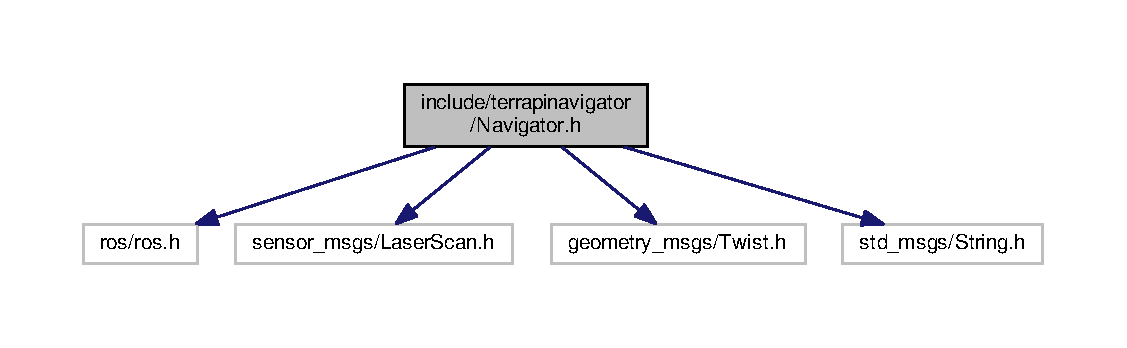
\includegraphics[width=350pt]{Navigator_8h__incl}
\end{center}
\end{figure}
This graph shows which files directly or indirectly include this file\+:
\nopagebreak
\begin{figure}[H]
\begin{center}
\leavevmode
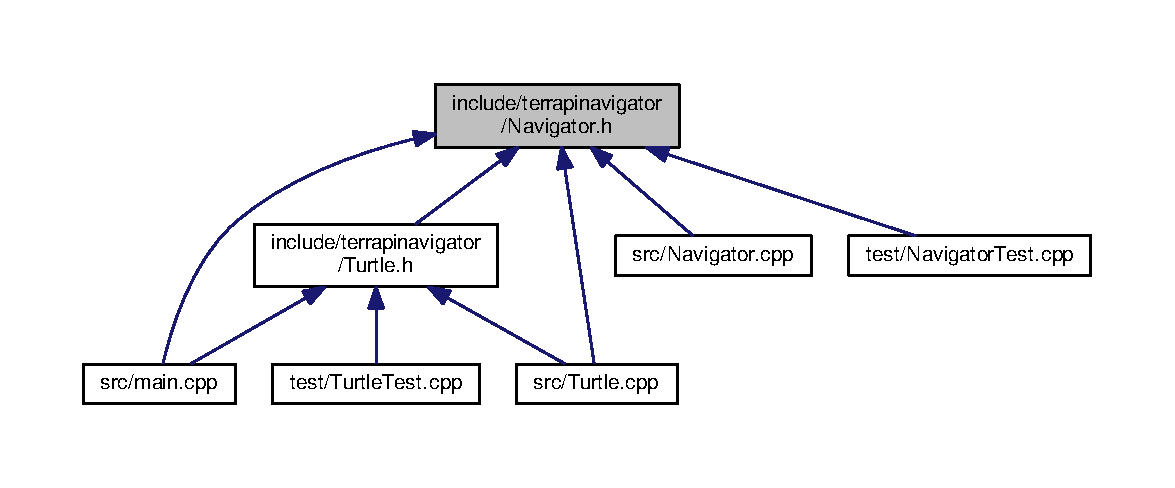
\includegraphics[width=350pt]{Navigator_8h__dep__incl}
\end{center}
\end{figure}
\subsection*{Classes}
\begin{DoxyCompactItemize}
\item 
class \hyperlink{classNavigator}{Navigator}
\begin{DoxyCompactList}\small\item\em \hyperlink{classNavigator}{Navigator} class. \end{DoxyCompactList}\end{DoxyCompactItemize}


\subsection{Detailed Description}
Header file of \hyperlink{classNavigator}{Navigator} class. 

\begin{DoxyAuthor}{Author}
Pranav Inani 
\end{DoxyAuthor}
\begin{DoxyCopyright}{Copyright}
2017 
\end{DoxyCopyright}

\hypertarget{TerpCam_8h}{}\section{include/terrapinavigator/\+Terp\+Cam.h File Reference}
\label{TerpCam_8h}\index{include/terrapinavigator/\+Terp\+Cam.\+h@{include/terrapinavigator/\+Terp\+Cam.\+h}}


Header file for \hyperlink{classTerpCam}{Terp\+Cam} class.  


{\ttfamily \#include $<$ros/ros.\+h$>$}\\*
{\ttfamily \#include $<$string$>$}\\*
{\ttfamily \#include $<$vector$>$}\\*
{\ttfamily \#include $<$iostream$>$}\\*
{\ttfamily \#include $<$terrapinavigator/picture\+Service.\+h$>$}\\*
{\ttfamily \#include $<$sensor\+\_\+msgs/\+Image.\+h$>$}\\*
Include dependency graph for Terp\+Cam.\+h\+:\nopagebreak
\begin{figure}[H]
\begin{center}
\leavevmode
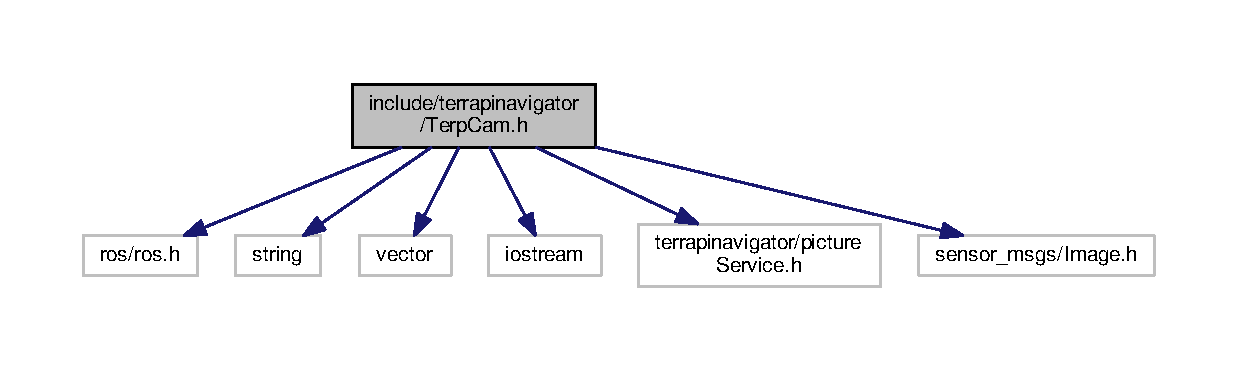
\includegraphics[width=350pt]{TerpCam_8h__incl}
\end{center}
\end{figure}
This graph shows which files directly or indirectly include this file\+:\nopagebreak
\begin{figure}[H]
\begin{center}
\leavevmode
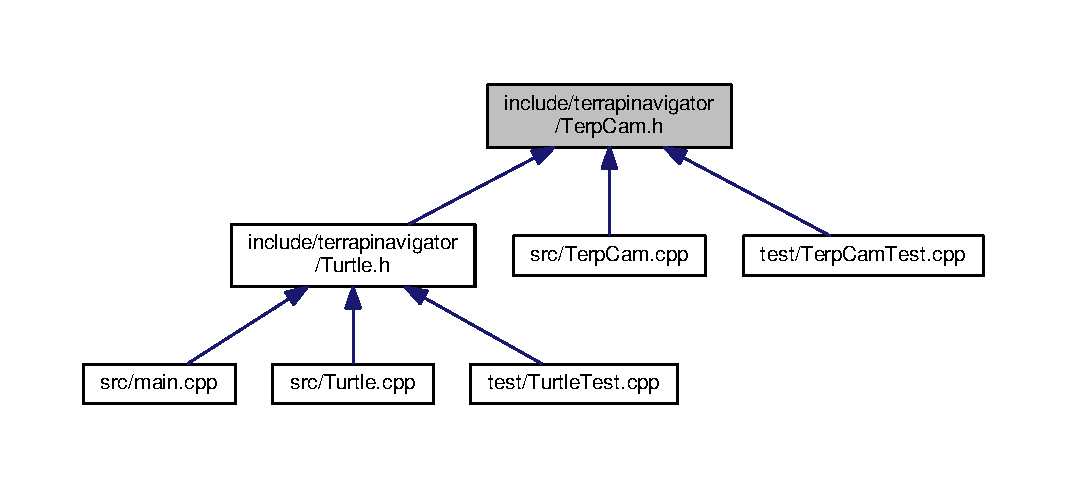
\includegraphics[width=350pt]{TerpCam_8h__dep__incl}
\end{center}
\end{figure}
\subsection*{Classes}
\begin{DoxyCompactItemize}
\item 
class \hyperlink{classTerpCam}{Terp\+Cam}
\begin{DoxyCompactList}\small\item\em \hyperlink{classTerpCam}{Terp\+Cam} class. \end{DoxyCompactList}\end{DoxyCompactItemize}


\subsection{Detailed Description}
Header file for \hyperlink{classTerpCam}{Terp\+Cam} class. 

\begin{DoxyAuthor}{Author}
Pranav Inani 
\end{DoxyAuthor}
\begin{DoxyCopyright}{Copyright}
2017 
\end{DoxyCopyright}

\hypertarget{Turtle_8h}{}\section{include/terrapinavigator/\+Turtle.h File Reference}
\label{Turtle_8h}\index{include/terrapinavigator/\+Turtle.\+h@{include/terrapinavigator/\+Turtle.\+h}}


Header File for turtle Class.  


{\ttfamily \#include \char`\"{}terrapinavigator/\+Navigator.\+h\char`\"{}}\\*
{\ttfamily \#include $<$terrapinavigator/picture\+Service.\+h$>$}\\*
{\ttfamily \#include \char`\"{}Terp\+Cam.\+h\char`\"{}}\\*
Include dependency graph for Turtle.\+h\+:
\nopagebreak
\begin{figure}[H]
\begin{center}
\leavevmode
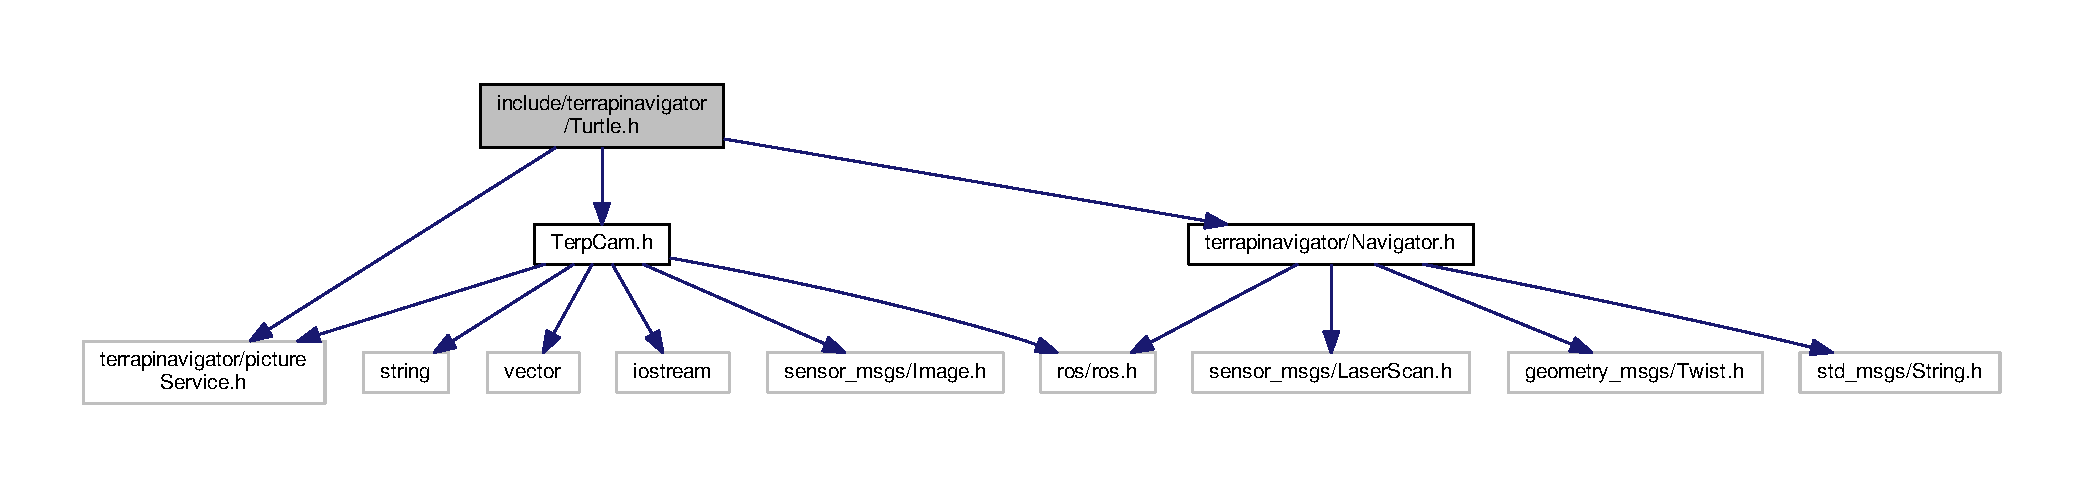
\includegraphics[width=350pt]{Turtle_8h__incl}
\end{center}
\end{figure}
This graph shows which files directly or indirectly include this file\+:\nopagebreak
\begin{figure}[H]
\begin{center}
\leavevmode
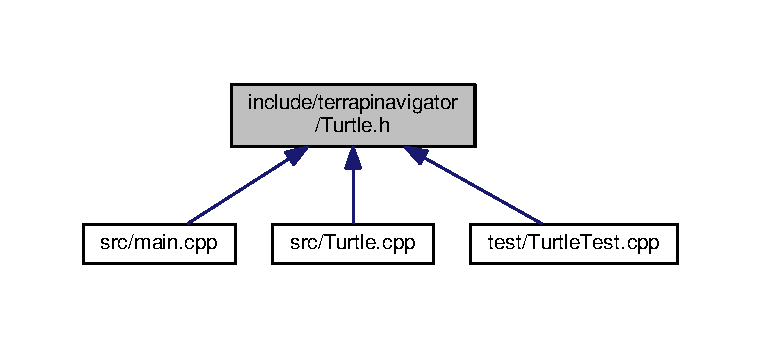
\includegraphics[width=350pt]{Turtle_8h__dep__incl}
\end{center}
\end{figure}
\subsection*{Classes}
\begin{DoxyCompactItemize}
\item 
class \hyperlink{classTurtle}{Turtle}
\begin{DoxyCompactList}\small\item\em \hyperlink{classTurtle}{Turtle} class. \end{DoxyCompactList}\end{DoxyCompactItemize}


\subsection{Detailed Description}
Header File for turtle Class. 

\begin{DoxyAuthor}{Author}
Pranav Inani 
\end{DoxyAuthor}
\begin{DoxyCopyright}{Copyright}
2017 
\end{DoxyCopyright}

\hypertarget{main_8cpp}{}\section{src/main.cpp File Reference}
\label{main_8cpp}\index{src/main.\+cpp@{src/main.\+cpp}}


Demo for the project.  


{\ttfamily \#include \char`\"{}ros/ros.\+h\char`\"{}}\\*
{\ttfamily \#include \char`\"{}std\+\_\+msgs/\+String.\+h\char`\"{}}\\*
{\ttfamily \#include \char`\"{}sensor\+\_\+msgs/\+Laser\+Scan.\+h\char`\"{}}\\*
{\ttfamily \#include \char`\"{}geometry\+\_\+msgs/\+Twist.\+h\char`\"{}}\\*
{\ttfamily \#include \char`\"{}terrapinavigator/\+Navigator.\+h\char`\"{}}\\*
{\ttfamily \#include \char`\"{}../include/terrapinavigator/\+Turtle.\+h\char`\"{}}\\*
Include dependency graph for main.\+cpp\+:
\nopagebreak
\begin{figure}[H]
\begin{center}
\leavevmode
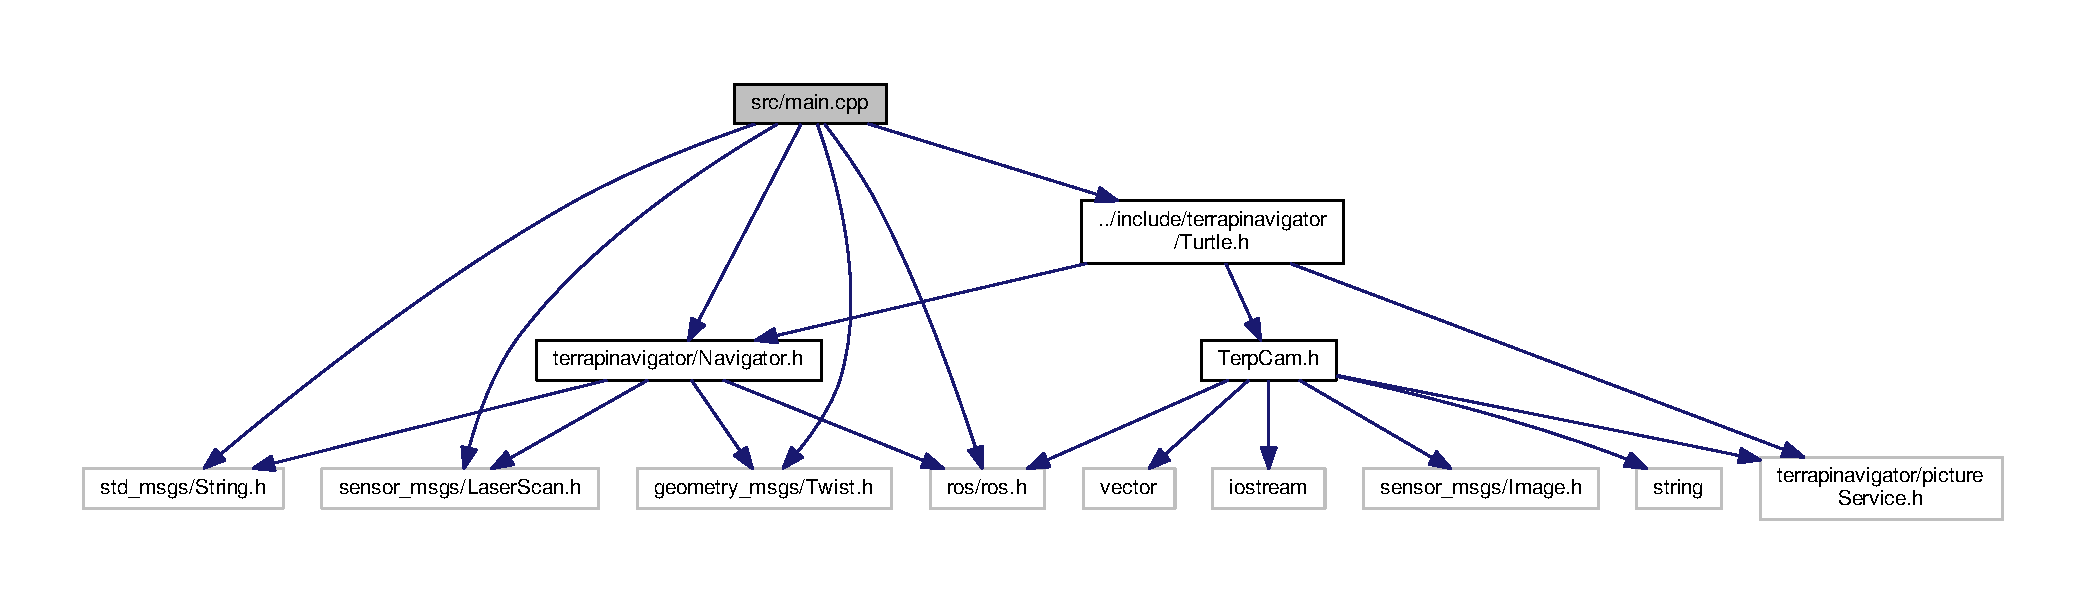
\includegraphics[width=350pt]{main_8cpp__incl}
\end{center}
\end{figure}
\subsection*{Functions}
\begin{DoxyCompactItemize}
\item 
int \hyperlink{main_8cpp_a3c04138a5bfe5d72780bb7e82a18e627}{main} (int argc, char $\ast$$\ast$argv)
\begin{DoxyCompactList}\small\item\em main function that demos the project \end{DoxyCompactList}\end{DoxyCompactItemize}


\subsection{Detailed Description}
Demo for the project. 

\begin{DoxyAuthor}{Author}
Pranav Inani 
\end{DoxyAuthor}
\begin{DoxyCopyright}{Copyright}
2017 
\end{DoxyCopyright}


\subsection{Function Documentation}
\index{main.\+cpp@{main.\+cpp}!main@{main}}
\index{main@{main}!main.\+cpp@{main.\+cpp}}
\subsubsection[{\texorpdfstring{main(int argc, char $\ast$$\ast$argv)}{main(int argc, char **argv)}}]{\setlength{\rightskip}{0pt plus 5cm}int main (
\begin{DoxyParamCaption}
\item[{int}]{argc, }
\item[{char $\ast$$\ast$}]{argv}
\end{DoxyParamCaption}
)}\hypertarget{main_8cpp_a3c04138a5bfe5d72780bb7e82a18e627}{}\label{main_8cpp_a3c04138a5bfe5d72780bb7e82a18e627}


main function that demos the project 


\begin{DoxyParams}{Parameters}
{\em argc} & is the argument count \\
\hline
{\em argv} & is the argument vector\\
\hline
\end{DoxyParams}
\begin{DoxyReturn}{Returns}
0 if all tests pass else 1 
\end{DoxyReturn}

\hypertarget{Navigator_8cpp}{}\section{src/\+Navigator.cpp File Reference}
\label{Navigator_8cpp}\index{src/\+Navigator.\+cpp@{src/\+Navigator.\+cpp}}


Implementation of \hyperlink{classNavigator}{Navigator} class.  


{\ttfamily \#include \char`\"{}ros/ros.\+h\char`\"{}}\\*
{\ttfamily \#include \char`\"{}std\+\_\+msgs/\+String.\+h\char`\"{}}\\*
{\ttfamily \#include \char`\"{}sensor\+\_\+msgs/\+Laser\+Scan.\+h\char`\"{}}\\*
{\ttfamily \#include \char`\"{}geometry\+\_\+msgs/\+Twist.\+h\char`\"{}}\\*
{\ttfamily \#include \char`\"{}terrapinavigator/\+Navigator.\+h\char`\"{}}\\*
Include dependency graph for Navigator.\+cpp\+:
\nopagebreak
\begin{figure}[H]
\begin{center}
\leavevmode
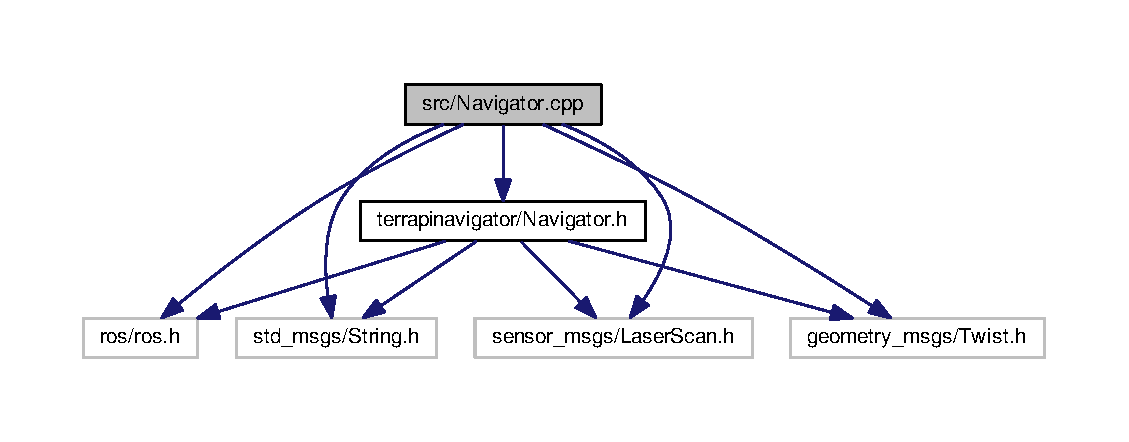
\includegraphics[width=350pt]{Navigator_8cpp__incl}
\end{center}
\end{figure}


\subsection{Detailed Description}
Implementation of \hyperlink{classNavigator}{Navigator} class. 

\begin{DoxyAuthor}{Author}
Pranav Inani 
\end{DoxyAuthor}
\begin{DoxyCopyright}{Copyright}
2017 
\end{DoxyCopyright}

\hypertarget{TerpCam_8cpp}{}\section{src/\+Terp\+Cam.cpp File Reference}
\label{TerpCam_8cpp}\index{src/\+Terp\+Cam.\+cpp@{src/\+Terp\+Cam.\+cpp}}


Implementation of \hyperlink{classTerpCam}{Terp\+Cam} class.  


{\ttfamily \#include $<$ros/ros.\+h$>$}\\*
{\ttfamily \#include $<$stdlib.\+h$>$}\\*
{\ttfamily \#include $<$cv\+\_\+bridge/cv\+\_\+bridge.\+h$>$}\\*
{\ttfamily \#include $<$sensor\+\_\+msgs/image\+\_\+encodings.\+h$>$}\\*
{\ttfamily \#include $<$image\+\_\+transport/image\+\_\+transport.\+h$>$}\\*
{\ttfamily \#include $<$sstream$>$}\\*
{\ttfamily \#include $<$string$>$}\\*
{\ttfamily \#include \char`\"{}terrapinavigator/picture\+Service.\+h\char`\"{}}\\*
{\ttfamily \#include \char`\"{}terrapinavigator/\+Terp\+Cam.\+h\char`\"{}}\\*
{\ttfamily \#include $<$opencv2/imgproc/imgproc.\+hpp$>$}\\*
{\ttfamily \#include $<$opencv2/core/core.\+hpp$>$}\\*
{\ttfamily \#include $<$opencv2/highgui/highgui.\+hpp$>$}\\*
Include dependency graph for Terp\+Cam.\+cpp\+:\nopagebreak
\begin{figure}[H]
\begin{center}
\leavevmode
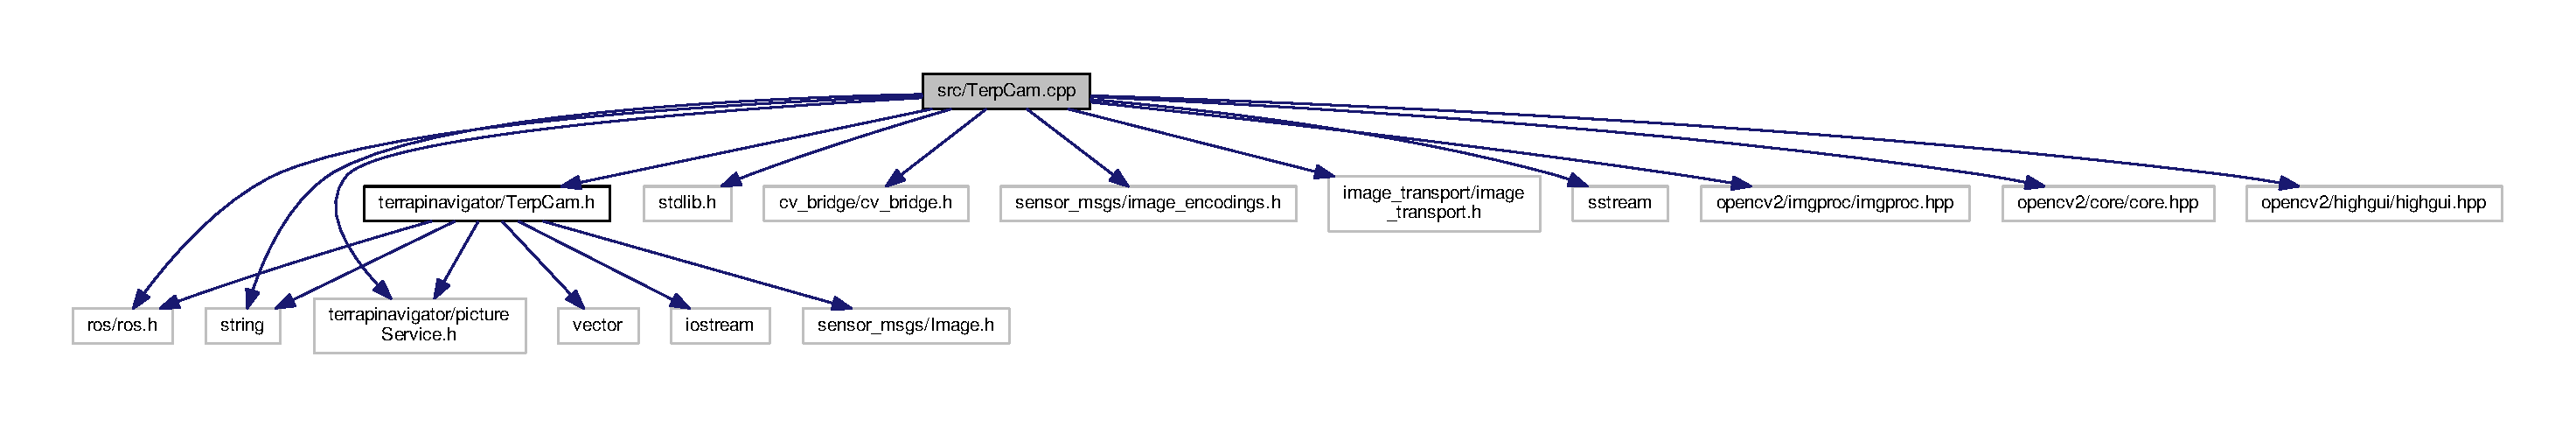
\includegraphics[width=350pt]{TerpCam_8cpp__incl}
\end{center}
\end{figure}


\subsection{Detailed Description}
Implementation of \hyperlink{classTerpCam}{Terp\+Cam} class. 

\begin{DoxyAuthor}{Author}
Pranav Inani 
\end{DoxyAuthor}
\begin{DoxyCopyright}{Copyright}
2017 
\end{DoxyCopyright}

\hypertarget{Turtle_8cpp}{}\section{src/\+Turtle.cpp File Reference}
\label{Turtle_8cpp}\index{src/\+Turtle.\+cpp@{src/\+Turtle.\+cpp}}


Implementation of \hyperlink{classTurtle}{Turtle} class.  


{\ttfamily \#include \char`\"{}terrapinavigator/\+Turtle.\+h\char`\"{}}\\*
{\ttfamily \#include $<$terrapinavigator/picture\+Service.\+h$>$}\\*
{\ttfamily \#include $<$ros/ros.\+h$>$}\\*
{\ttfamily \#include $<$iostream$>$}\\*
{\ttfamily \#include \char`\"{}terrapinavigator/\+Navigator.\+h\char`\"{}}\\*
Include dependency graph for Turtle.\+cpp\+:
\nopagebreak
\begin{figure}[H]
\begin{center}
\leavevmode
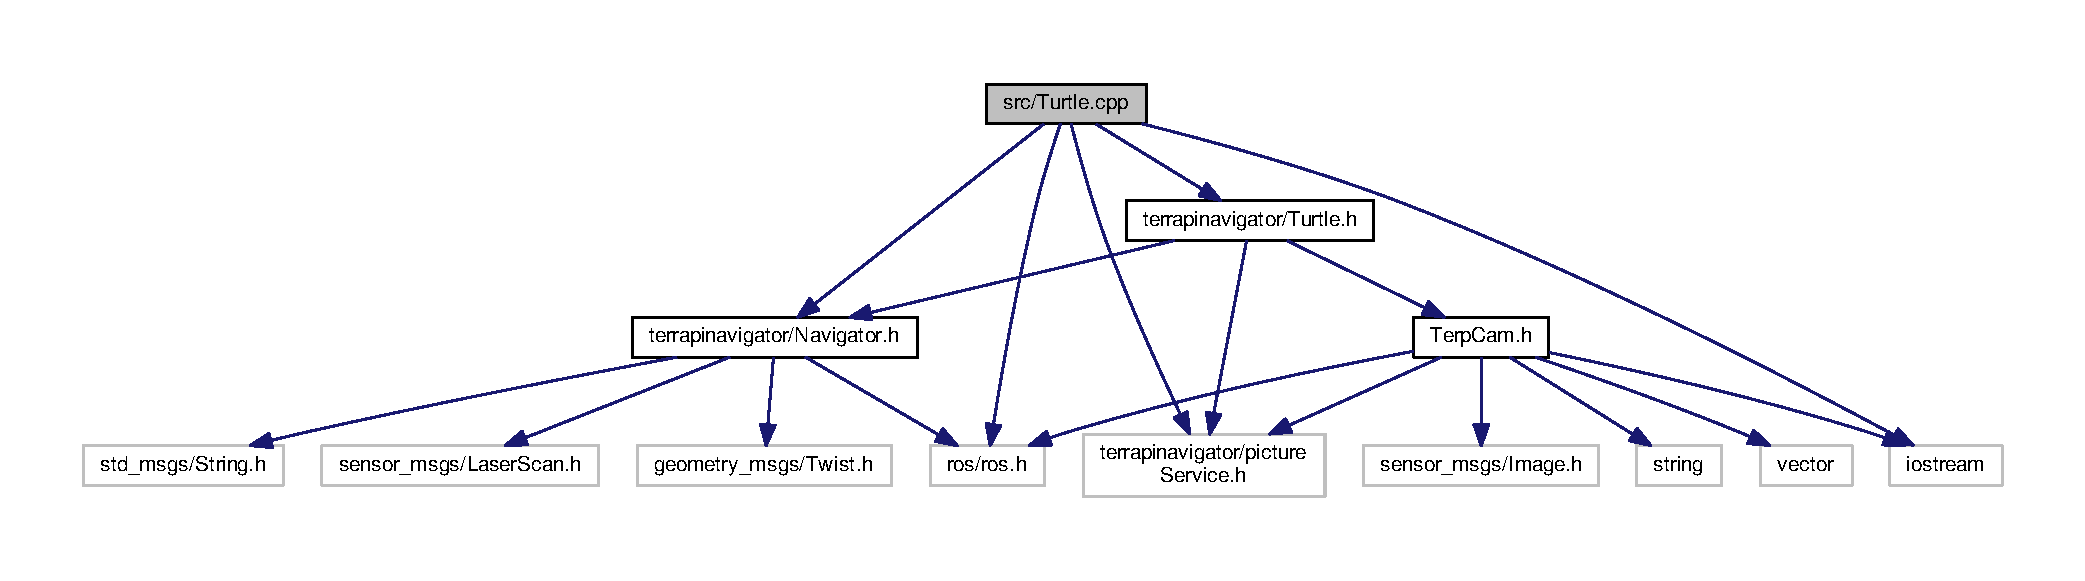
\includegraphics[width=350pt]{Turtle_8cpp__incl}
\end{center}
\end{figure}


\subsection{Detailed Description}
Implementation of \hyperlink{classTurtle}{Turtle} class. 

\begin{DoxyAuthor}{Author}
Pranav Inani 
\end{DoxyAuthor}
\begin{DoxyCopyright}{Copyright}
2017 
\end{DoxyCopyright}

\hypertarget{NavigatorTest_8cpp}{}\section{test/\+Navigator\+Test.cpp File Reference}
\label{NavigatorTest_8cpp}\index{test/\+Navigator\+Test.\+cpp@{test/\+Navigator\+Test.\+cpp}}


Contains tests for navigator class.  


{\ttfamily \#include $<$ros/ros.\+h$>$}\\*
{\ttfamily \#include $<$gtest/gtest.\+h$>$}\\*
{\ttfamily \#include \char`\"{}terrapinavigator/\+Navigator.\+h\char`\"{}}\\*
Include dependency graph for Navigator\+Test.\+cpp\+:
\nopagebreak
\begin{figure}[H]
\begin{center}
\leavevmode
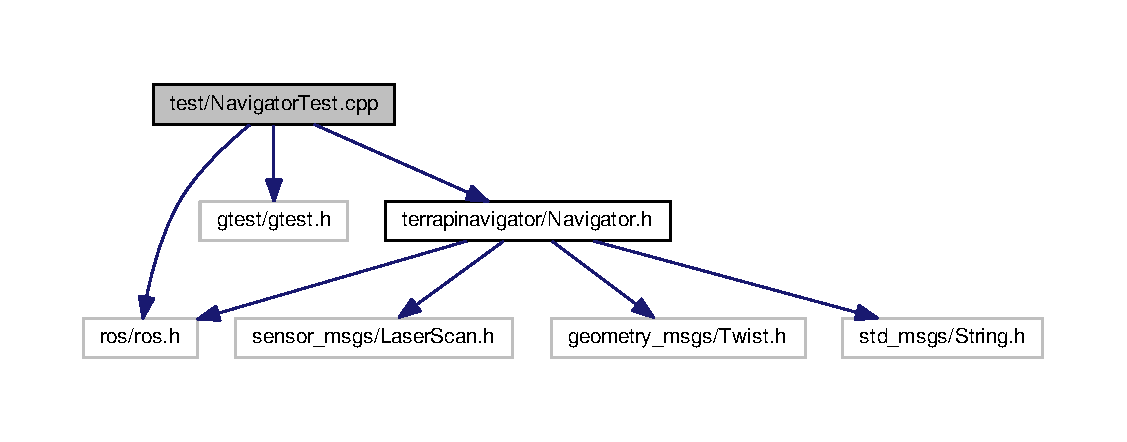
\includegraphics[width=350pt]{NavigatorTest_8cpp__incl}
\end{center}
\end{figure}
\subsection*{Functions}
\begin{DoxyCompactItemize}
\item 
\hyperlink{NavigatorTest_8cpp_a33d8c1e575420cc79b1427a3daa1d04a}{T\+E\+ST} (Navigator\+Test, Initial\+Linear\+Test)
\begin{DoxyCompactList}\small\item\em Unit test to check initial linear motion. \end{DoxyCompactList}\item 
\hyperlink{NavigatorTest_8cpp_a9c41f074f8c452de6639c8d057bdd553}{T\+E\+ST} (Navigator\+Test, Initial\+Angular\+Test)
\begin{DoxyCompactList}\small\item\em Unit test to check initial angular rotation. \end{DoxyCompactList}\item 
\hyperlink{NavigatorTest_8cpp_ab7b68c9d72fabd287db8797fad51ad5c}{T\+E\+ST} (Navigator\+Test, Callback\+Test)
\begin{DoxyCompactList}\small\item\em Unit test for scan callback. \end{DoxyCompactList}\item 
\hyperlink{NavigatorTest_8cpp_a873560fb9d7c6efcd756e32442e74f4e}{T\+E\+ST} (Navigator\+Test, Rotate\+Flag\+Test)
\begin{DoxyCompactList}\small\item\em Unit test for rotate flag. \end{DoxyCompactList}\item 
\hyperlink{NavigatorTest_8cpp_a9848cdb9a04916d83808ba14c6d54538}{T\+E\+ST} (Navigator\+Test, Initial\+Rotate\+Test)
\begin{DoxyCompactList}\small\item\em Unit test to check timer callback functionality. \end{DoxyCompactList}\item 
\hyperlink{NavigatorTest_8cpp_a76f1622e33d5f843416c2ea6b65c69f0}{T\+E\+ST} (Navigator\+Test, Random\+Angle\+Test)
\begin{DoxyCompactList}\small\item\em Unit test for random angle rotation. \end{DoxyCompactList}\end{DoxyCompactItemize}


\subsection{Detailed Description}
Contains tests for navigator class. 

\begin{DoxyAuthor}{Author}
Pranav Inani 
\end{DoxyAuthor}
\begin{DoxyCopyright}{Copyright}
2017 
\end{DoxyCopyright}


\subsection{Function Documentation}
\index{Navigator\+Test.\+cpp@{Navigator\+Test.\+cpp}!T\+E\+ST@{T\+E\+ST}}
\index{T\+E\+ST@{T\+E\+ST}!Navigator\+Test.\+cpp@{Navigator\+Test.\+cpp}}
\subsubsection[{\texorpdfstring{T\+E\+S\+T(\+Navigator\+Test, Initial\+Linear\+Test)}{TEST(NavigatorTest, InitialLinearTest)}}]{\setlength{\rightskip}{0pt plus 5cm}T\+E\+ST (
\begin{DoxyParamCaption}
\item[{Navigator\+Test}]{, }
\item[{Initial\+Linear\+Test}]{}
\end{DoxyParamCaption}
)}\hypertarget{NavigatorTest_8cpp_a33d8c1e575420cc79b1427a3daa1d04a}{}\label{NavigatorTest_8cpp_a33d8c1e575420cc79b1427a3daa1d04a}


Unit test to check initial linear motion. 

Checks if the turtlebot has no movement in x direction as we only want it to rotate initially \index{Navigator\+Test.\+cpp@{Navigator\+Test.\+cpp}!T\+E\+ST@{T\+E\+ST}}
\index{T\+E\+ST@{T\+E\+ST}!Navigator\+Test.\+cpp@{Navigator\+Test.\+cpp}}
\subsubsection[{\texorpdfstring{T\+E\+S\+T(\+Navigator\+Test, Initial\+Angular\+Test)}{TEST(NavigatorTest, InitialAngularTest)}}]{\setlength{\rightskip}{0pt plus 5cm}T\+E\+ST (
\begin{DoxyParamCaption}
\item[{Navigator\+Test}]{, }
\item[{Initial\+Angular\+Test}]{}
\end{DoxyParamCaption}
)}\hypertarget{NavigatorTest_8cpp_a9c41f074f8c452de6639c8d057bdd553}{}\label{NavigatorTest_8cpp_a9c41f074f8c452de6639c8d057bdd553}


Unit test to check initial angular rotation. 

Checks if the action initially is to rotate the turtlebot in place to explore environment \index{Navigator\+Test.\+cpp@{Navigator\+Test.\+cpp}!T\+E\+ST@{T\+E\+ST}}
\index{T\+E\+ST@{T\+E\+ST}!Navigator\+Test.\+cpp@{Navigator\+Test.\+cpp}}
\subsubsection[{\texorpdfstring{T\+E\+S\+T(\+Navigator\+Test, Callback\+Test)}{TEST(NavigatorTest, CallbackTest)}}]{\setlength{\rightskip}{0pt plus 5cm}T\+E\+ST (
\begin{DoxyParamCaption}
\item[{Navigator\+Test}]{, }
\item[{Callback\+Test}]{}
\end{DoxyParamCaption}
)}\hypertarget{NavigatorTest_8cpp_ab7b68c9d72fabd287db8797fad51ad5c}{}\label{NavigatorTest_8cpp_ab7b68c9d72fabd287db8797fad51ad5c}


Unit test for scan callback. 

Checks if the obstacle distance is in the desired range \index{Navigator\+Test.\+cpp@{Navigator\+Test.\+cpp}!T\+E\+ST@{T\+E\+ST}}
\index{T\+E\+ST@{T\+E\+ST}!Navigator\+Test.\+cpp@{Navigator\+Test.\+cpp}}
\subsubsection[{\texorpdfstring{T\+E\+S\+T(\+Navigator\+Test, Rotate\+Flag\+Test)}{TEST(NavigatorTest, RotateFlagTest)}}]{\setlength{\rightskip}{0pt plus 5cm}T\+E\+ST (
\begin{DoxyParamCaption}
\item[{Navigator\+Test}]{, }
\item[{Rotate\+Flag\+Test}]{}
\end{DoxyParamCaption}
)}\hypertarget{NavigatorTest_8cpp_a873560fb9d7c6efcd756e32442e74f4e}{}\label{NavigatorTest_8cpp_a873560fb9d7c6efcd756e32442e74f4e}


Unit test for rotate flag. 

Checks the setter and getter for rotate flag \index{Navigator\+Test.\+cpp@{Navigator\+Test.\+cpp}!T\+E\+ST@{T\+E\+ST}}
\index{T\+E\+ST@{T\+E\+ST}!Navigator\+Test.\+cpp@{Navigator\+Test.\+cpp}}
\subsubsection[{\texorpdfstring{T\+E\+S\+T(\+Navigator\+Test, Initial\+Rotate\+Test)}{TEST(NavigatorTest, InitialRotateTest)}}]{\setlength{\rightskip}{0pt plus 5cm}T\+E\+ST (
\begin{DoxyParamCaption}
\item[{Navigator\+Test}]{, }
\item[{Initial\+Rotate\+Test}]{}
\end{DoxyParamCaption}
)}\hypertarget{NavigatorTest_8cpp_a9848cdb9a04916d83808ba14c6d54538}{}\label{NavigatorTest_8cpp_a9848cdb9a04916d83808ba14c6d54538}


Unit test to check timer callback functionality. 

Checks if the timer callback was called and the necessary flag was set \index{Navigator\+Test.\+cpp@{Navigator\+Test.\+cpp}!T\+E\+ST@{T\+E\+ST}}
\index{T\+E\+ST@{T\+E\+ST}!Navigator\+Test.\+cpp@{Navigator\+Test.\+cpp}}
\subsubsection[{\texorpdfstring{T\+E\+S\+T(\+Navigator\+Test, Random\+Angle\+Test)}{TEST(NavigatorTest, RandomAngleTest)}}]{\setlength{\rightskip}{0pt plus 5cm}T\+E\+ST (
\begin{DoxyParamCaption}
\item[{Navigator\+Test}]{, }
\item[{Random\+Angle\+Test}]{}
\end{DoxyParamCaption}
)}\hypertarget{NavigatorTest_8cpp_a76f1622e33d5f843416c2ea6b65c69f0}{}\label{NavigatorTest_8cpp_a76f1622e33d5f843416c2ea6b65c69f0}


Unit test for random angle rotation. 

Checks if the robot moves with the desired range of random angle when obstacle is detected 
\hypertarget{TerpCamTest_8cpp}{}\section{test/\+Terp\+Cam\+Test.cpp File Reference}
\label{TerpCamTest_8cpp}\index{test/\+Terp\+Cam\+Test.\+cpp@{test/\+Terp\+Cam\+Test.\+cpp}}


Contains tests for \hyperlink{classTerpCam}{Terp\+Cam} class.  


{\ttfamily \#include $<$ros/ros.\+h$>$}\\*
{\ttfamily \#include $<$gtest/gtest.\+h$>$}\\*
{\ttfamily \#include \char`\"{}terrapinavigator/\+Terp\+Cam.\+h\char`\"{}}\\*
Include dependency graph for Terp\+Cam\+Test.\+cpp\+:\nopagebreak
\begin{figure}[H]
\begin{center}
\leavevmode
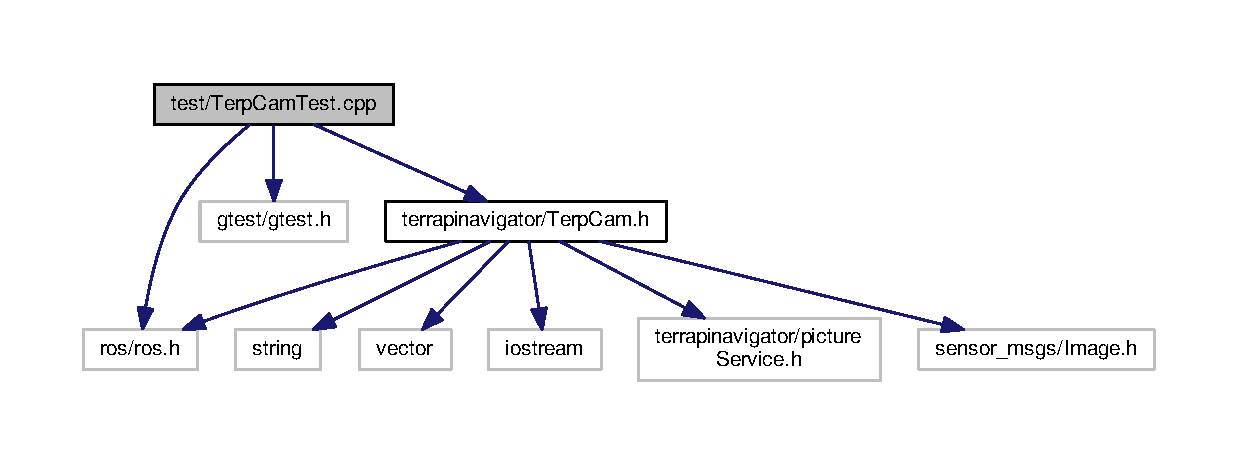
\includegraphics[width=350pt]{TerpCamTest_8cpp__incl}
\end{center}
\end{figure}
\subsection*{Functions}
\begin{DoxyCompactItemize}
\item 
\hyperlink{TerpCamTest_8cpp_ace8f0b0501dfb7d64f8b66ea2ebabb14}{T\+E\+ST} (Terp\+Cam\+Test, set\+Image\+Flag\+Test)
\begin{DoxyCompactList}\small\item\em Unit test for image flag. \end{DoxyCompactList}\item 
\hyperlink{TerpCamTest_8cpp_a13b36a16e604cbfcf9b2dec50906c77c}{T\+E\+ST} (Terp\+Cam\+Test, Initial\+Image\+Flag\+Test)
\begin{DoxyCompactList}\small\item\em Unit test for image flag. \end{DoxyCompactList}\end{DoxyCompactItemize}


\subsection{Detailed Description}
Contains tests for \hyperlink{classTerpCam}{Terp\+Cam} class. 

\begin{DoxyAuthor}{Author}
Pranav Inani 
\end{DoxyAuthor}
\begin{DoxyCopyright}{Copyright}
2017 
\end{DoxyCopyright}


\subsection{Function Documentation}
\index{Terp\+Cam\+Test.\+cpp@{Terp\+Cam\+Test.\+cpp}!T\+E\+ST@{T\+E\+ST}}
\index{T\+E\+ST@{T\+E\+ST}!Terp\+Cam\+Test.\+cpp@{Terp\+Cam\+Test.\+cpp}}
\subsubsection[{\texorpdfstring{T\+E\+S\+T(\+Terp\+Cam\+Test, set\+Image\+Flag\+Test)}{TEST(TerpCamTest, setImageFlagTest)}}]{\setlength{\rightskip}{0pt plus 5cm}T\+E\+ST (
\begin{DoxyParamCaption}
\item[{Terp\+Cam\+Test}]{, }
\item[{set\+Image\+Flag\+Test}]{}
\end{DoxyParamCaption}
)}\hypertarget{TerpCamTest_8cpp_ace8f0b0501dfb7d64f8b66ea2ebabb14}{}\label{TerpCamTest_8cpp_ace8f0b0501dfb7d64f8b66ea2ebabb14}


Unit test for image flag. 

Checks the setter and getter for rotate flag \index{Terp\+Cam\+Test.\+cpp@{Terp\+Cam\+Test.\+cpp}!T\+E\+ST@{T\+E\+ST}}
\index{T\+E\+ST@{T\+E\+ST}!Terp\+Cam\+Test.\+cpp@{Terp\+Cam\+Test.\+cpp}}
\subsubsection[{\texorpdfstring{T\+E\+S\+T(\+Terp\+Cam\+Test, Initial\+Image\+Flag\+Test)}{TEST(TerpCamTest, InitialImageFlagTest)}}]{\setlength{\rightskip}{0pt plus 5cm}T\+E\+ST (
\begin{DoxyParamCaption}
\item[{Terp\+Cam\+Test}]{, }
\item[{Initial\+Image\+Flag\+Test}]{}
\end{DoxyParamCaption}
)}\hypertarget{TerpCamTest_8cpp_a13b36a16e604cbfcf9b2dec50906c77c}{}\label{TerpCamTest_8cpp_a13b36a16e604cbfcf9b2dec50906c77c}


Unit test for image flag. 

Checks the inital condition of rotate flag 
\hypertarget{terpTest_8cpp}{}\section{test/terp\+Test.cpp File Reference}
\label{terpTest_8cpp}\index{test/terp\+Test.\+cpp@{test/terp\+Test.\+cpp}}


Contains the main function to run all tests.  


{\ttfamily \#include $<$ros/ros.\+h$>$}\\*
{\ttfamily \#include $<$gtest/gtest.\+h$>$}\\*
Include dependency graph for terp\+Test.\+cpp\+:
\nopagebreak
\begin{figure}[H]
\begin{center}
\leavevmode
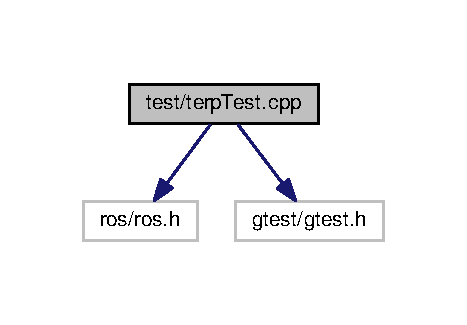
\includegraphics[width=224pt]{terpTest_8cpp__incl}
\end{center}
\end{figure}
\subsection*{Functions}
\begin{DoxyCompactItemize}
\item 
int \hyperlink{terpTest_8cpp_a3c04138a5bfe5d72780bb7e82a18e627}{main} (int argc, char $\ast$$\ast$argv)
\begin{DoxyCompactList}\small\item\em main function for running all google tests \end{DoxyCompactList}\end{DoxyCompactItemize}


\subsection{Detailed Description}
Contains the main function to run all tests. 

\begin{DoxyAuthor}{Author}
Pranav Inani 
\end{DoxyAuthor}
\begin{DoxyCopyright}{Copyright}
2017 
\end{DoxyCopyright}


\subsection{Function Documentation}
\index{terp\+Test.\+cpp@{terp\+Test.\+cpp}!main@{main}}
\index{main@{main}!terp\+Test.\+cpp@{terp\+Test.\+cpp}}
\subsubsection[{\texorpdfstring{main(int argc, char $\ast$$\ast$argv)}{main(int argc, char **argv)}}]{\setlength{\rightskip}{0pt plus 5cm}int main (
\begin{DoxyParamCaption}
\item[{int}]{argc, }
\item[{char $\ast$$\ast$}]{argv}
\end{DoxyParamCaption}
)}\hypertarget{terpTest_8cpp_a3c04138a5bfe5d72780bb7e82a18e627}{}\label{terpTest_8cpp_a3c04138a5bfe5d72780bb7e82a18e627}


main function for running all google tests 


\begin{DoxyParams}{Parameters}
{\em argc} & is the argument count \\
\hline
{\em argv} & is the argument vector\\
\hline
\end{DoxyParams}
\begin{DoxyReturn}{Returns}
0 if all tests pass else 1 
\end{DoxyReturn}

\hypertarget{TurtleTest_8cpp}{}\section{test/\+Turtle\+Test.cpp File Reference}
\label{TurtleTest_8cpp}\index{test/\+Turtle\+Test.\+cpp@{test/\+Turtle\+Test.\+cpp}}


Contains tests for \hyperlink{classTurtle}{Turtle} class.  


{\ttfamily \#include $<$ros/ros.\+h$>$}\\*
{\ttfamily \#include $<$gtest/gtest.\+h$>$}\\*
{\ttfamily \#include \char`\"{}../include/terrapinavigator/\+Turtle.\+h\char`\"{}}\\*
Include dependency graph for Turtle\+Test.\+cpp\+:
\nopagebreak
\begin{figure}[H]
\begin{center}
\leavevmode
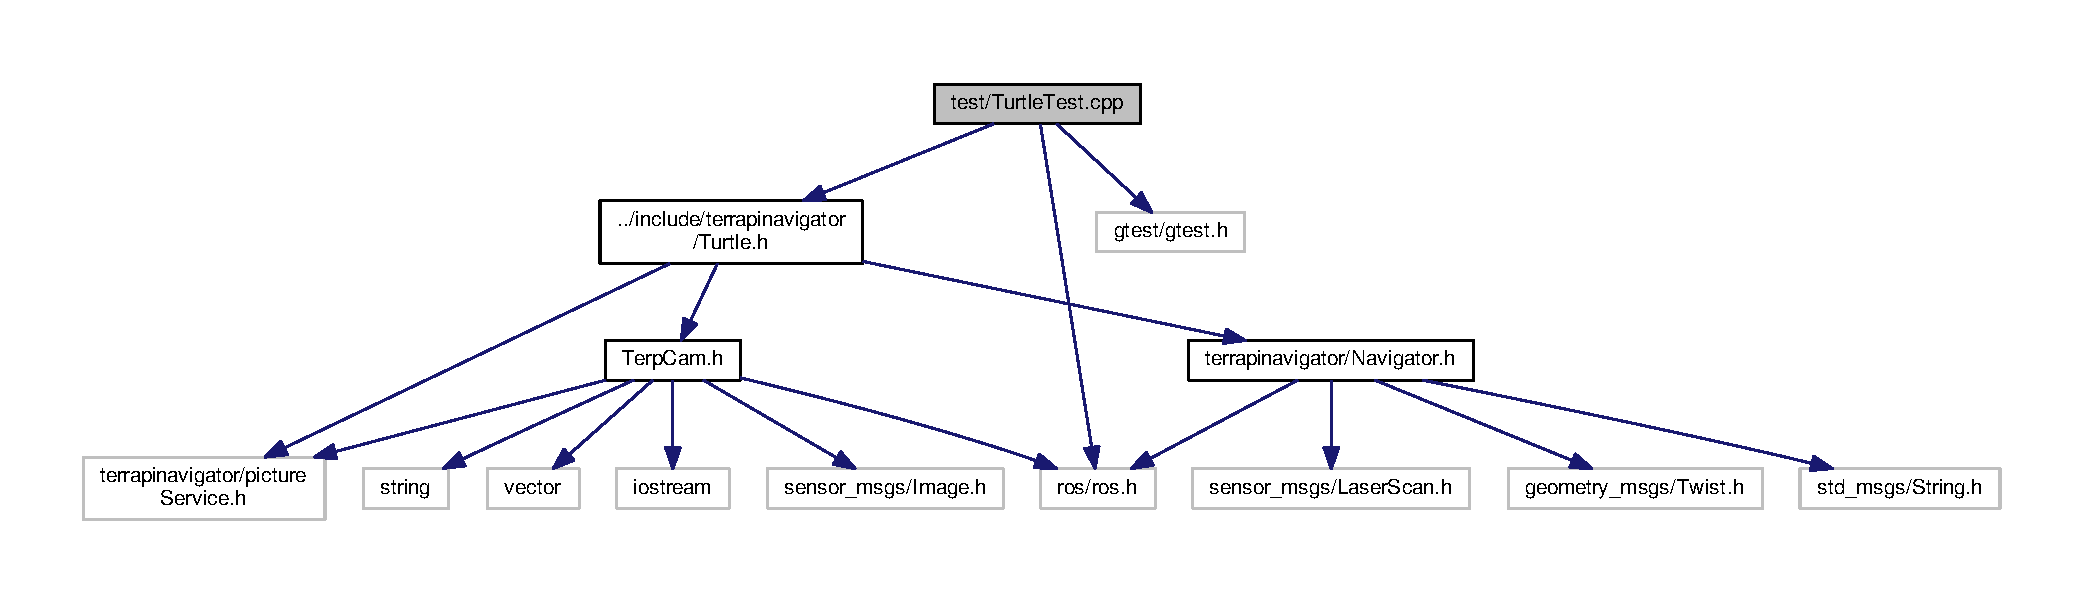
\includegraphics[width=350pt]{TurtleTest_8cpp__incl}
\end{center}
\end{figure}
\subsection*{Functions}
\begin{DoxyCompactItemize}
\item 
\hyperlink{TurtleTest_8cpp_a90bd3453baf37f4012e07e4d12ca1735}{T\+E\+ST} (Turtle\+Test, Publish\+Test)
\begin{DoxyCompactList}\small\item\em Unit test to check if messages are being publishes. \end{DoxyCompactList}\end{DoxyCompactItemize}


\subsection{Detailed Description}
Contains tests for \hyperlink{classTurtle}{Turtle} class. 

\begin{DoxyAuthor}{Author}
Pranav Inani 
\end{DoxyAuthor}
\begin{DoxyCopyright}{Copyright}
2017 
\end{DoxyCopyright}


\subsection{Function Documentation}
\index{Turtle\+Test.\+cpp@{Turtle\+Test.\+cpp}!T\+E\+ST@{T\+E\+ST}}
\index{T\+E\+ST@{T\+E\+ST}!Turtle\+Test.\+cpp@{Turtle\+Test.\+cpp}}
\subsubsection[{\texorpdfstring{T\+E\+S\+T(\+Turtle\+Test, Publish\+Test)}{TEST(TurtleTest, PublishTest)}}]{\setlength{\rightskip}{0pt plus 5cm}T\+E\+ST (
\begin{DoxyParamCaption}
\item[{Turtle\+Test}]{, }
\item[{Publish\+Test}]{}
\end{DoxyParamCaption}
)}\hypertarget{TurtleTest_8cpp_a90bd3453baf37f4012e07e4d12ca1735}{}\label{TurtleTest_8cpp_a90bd3453baf37f4012e07e4d12ca1735}


Unit test to check if messages are being publishes. 

Checks if the explore function is publishing twist messages 
%--- End generated contents ---

% Index
\backmatter
\newpage
\phantomsection
\clearemptydoublepage
\addcontentsline{toc}{chapter}{Index}
\printindex

\end{document}
